\section{Benchmarks}

Here, we present some benchmarks for the comparison of our implementation of the algorithm against the FLINT library for bivariate polynomial resultant computation.

All benchmarks presented below are performed on an Apple MacBook with 8-core Apple M2 SoC, 16 GB unified memory. All results are the average running time of 5 independent trials, and the bitsize of polynomial coefficients is fixed to be 50 in all cases.

Note that for our proposed implementation, we present 6 different running times, based on the selection method of points that are used to interpolate the polynomial:

\begin{enumerate}
  \item Random Points: Fully random points in the bitsize of polynomial coefficients.
  \item Random Positive Points: Fully random and positive points in the bitsize of polynomial coefficients.
  \item Small Random Points: Small random points in the bitsize of the degree of the polynomial.
  \item Small Random Positive Points: Small random and positive points in the bitsize of the degree of the polynomial.
  \item Ordered Points: Ordered points in the ascending order of bitsize.
  \item Ordered Positive Points: Ordered and positive points in the ascending order of bitsize.
\end{enumerate}

\subsection{Benchmarks for integer polynomials}

\begin{figure}[H]
  \centering
  \begin{subfigure}{0.70\textwidth}
    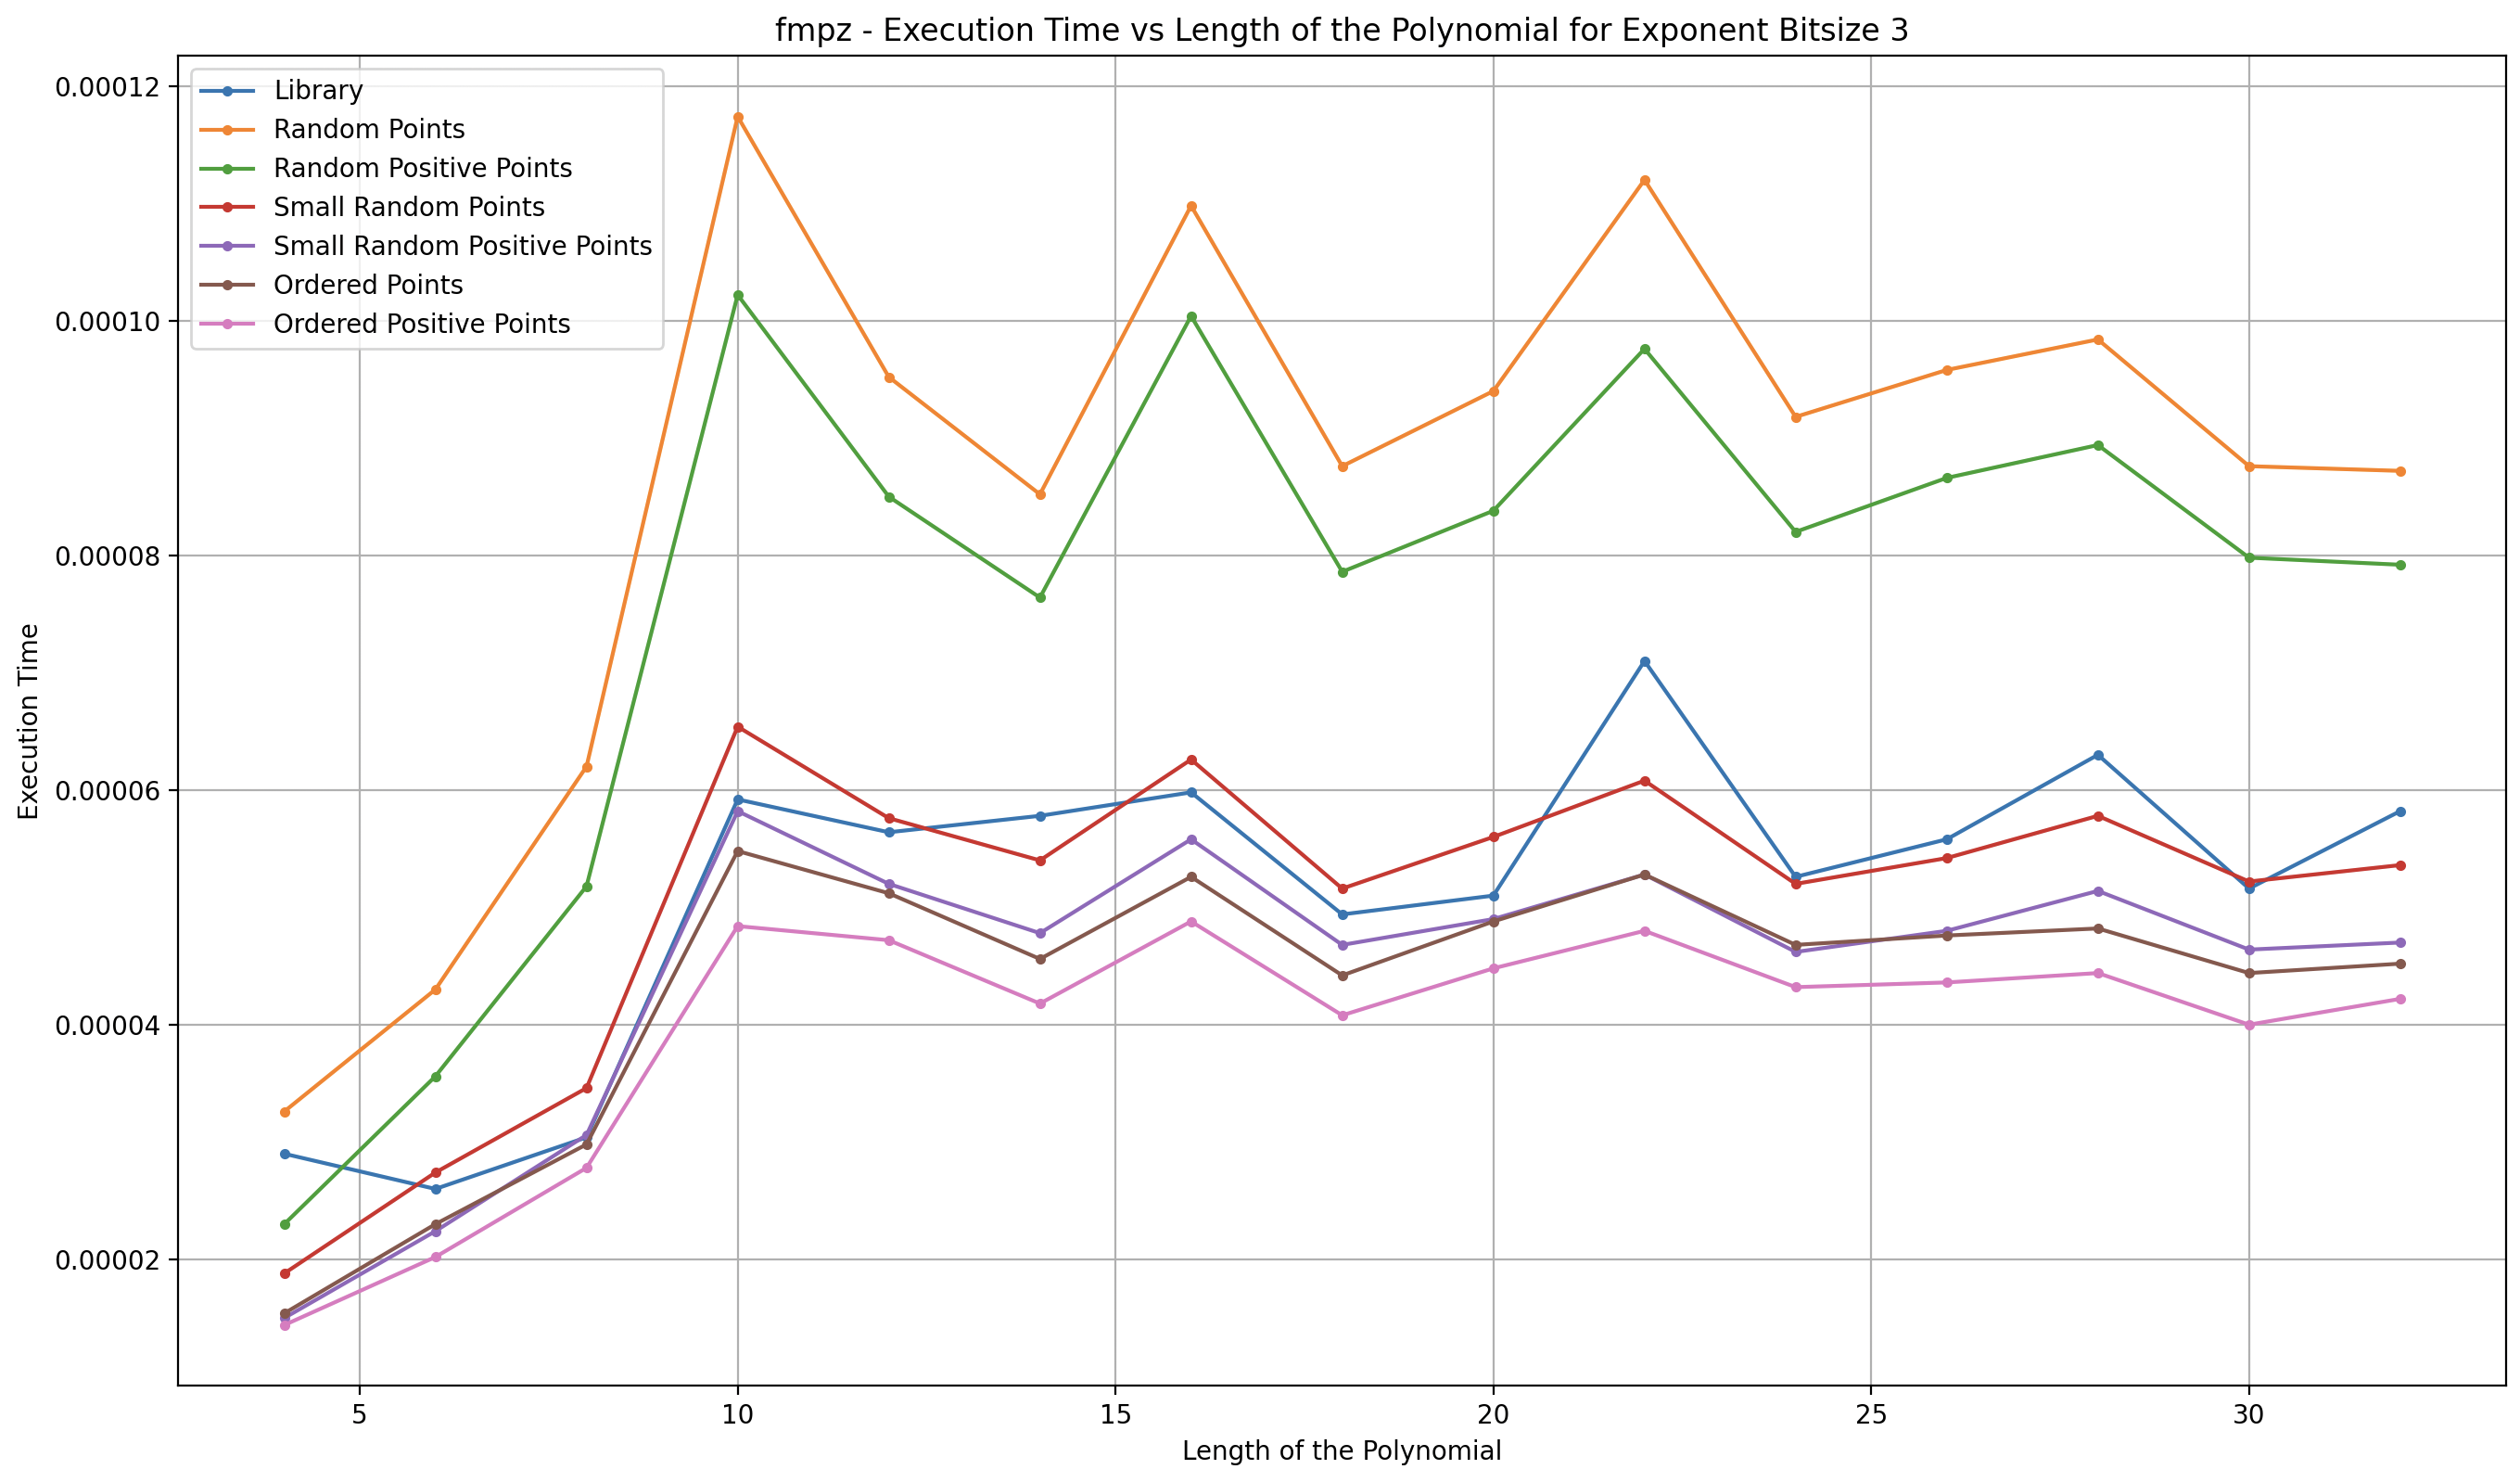
\includegraphics[width=\linewidth]{./images/fmpz_bitsize_3.png}
  \end{subfigure}
  \caption{FMPZ bivariate polynomial resultant execution time (in seconds) for exponent bitsize 3 with varying lengths.}
  \label{fig:benc.fmpz.3}
\end{figure}

In Figure \ref{fig:benc.fmpz.3}, we first compare our implementation against the library in small polynomials, i.e. of exponent bitsize 3. We see that while the random selection of points for the interpolation method is significantly slower than the rest, other methods have similar running times. This important difference between random selection and others can be explained by the bitsize of the points used in the interpolation. When a uniformly random selection is performed, bitsize of the points used in the interpolation is the same as the bitsize of coefficients, i.e. 50. Thus, the interpolation takes significantly more time than other approaches.

Another important observation, about rest of the measured methods, is that even though FLINT's implementation is slower in some cases, there is no important difference between their running times.

\begin{figure}[H]
  \centering
  \begin{subfigure}{0.45\textwidth}
    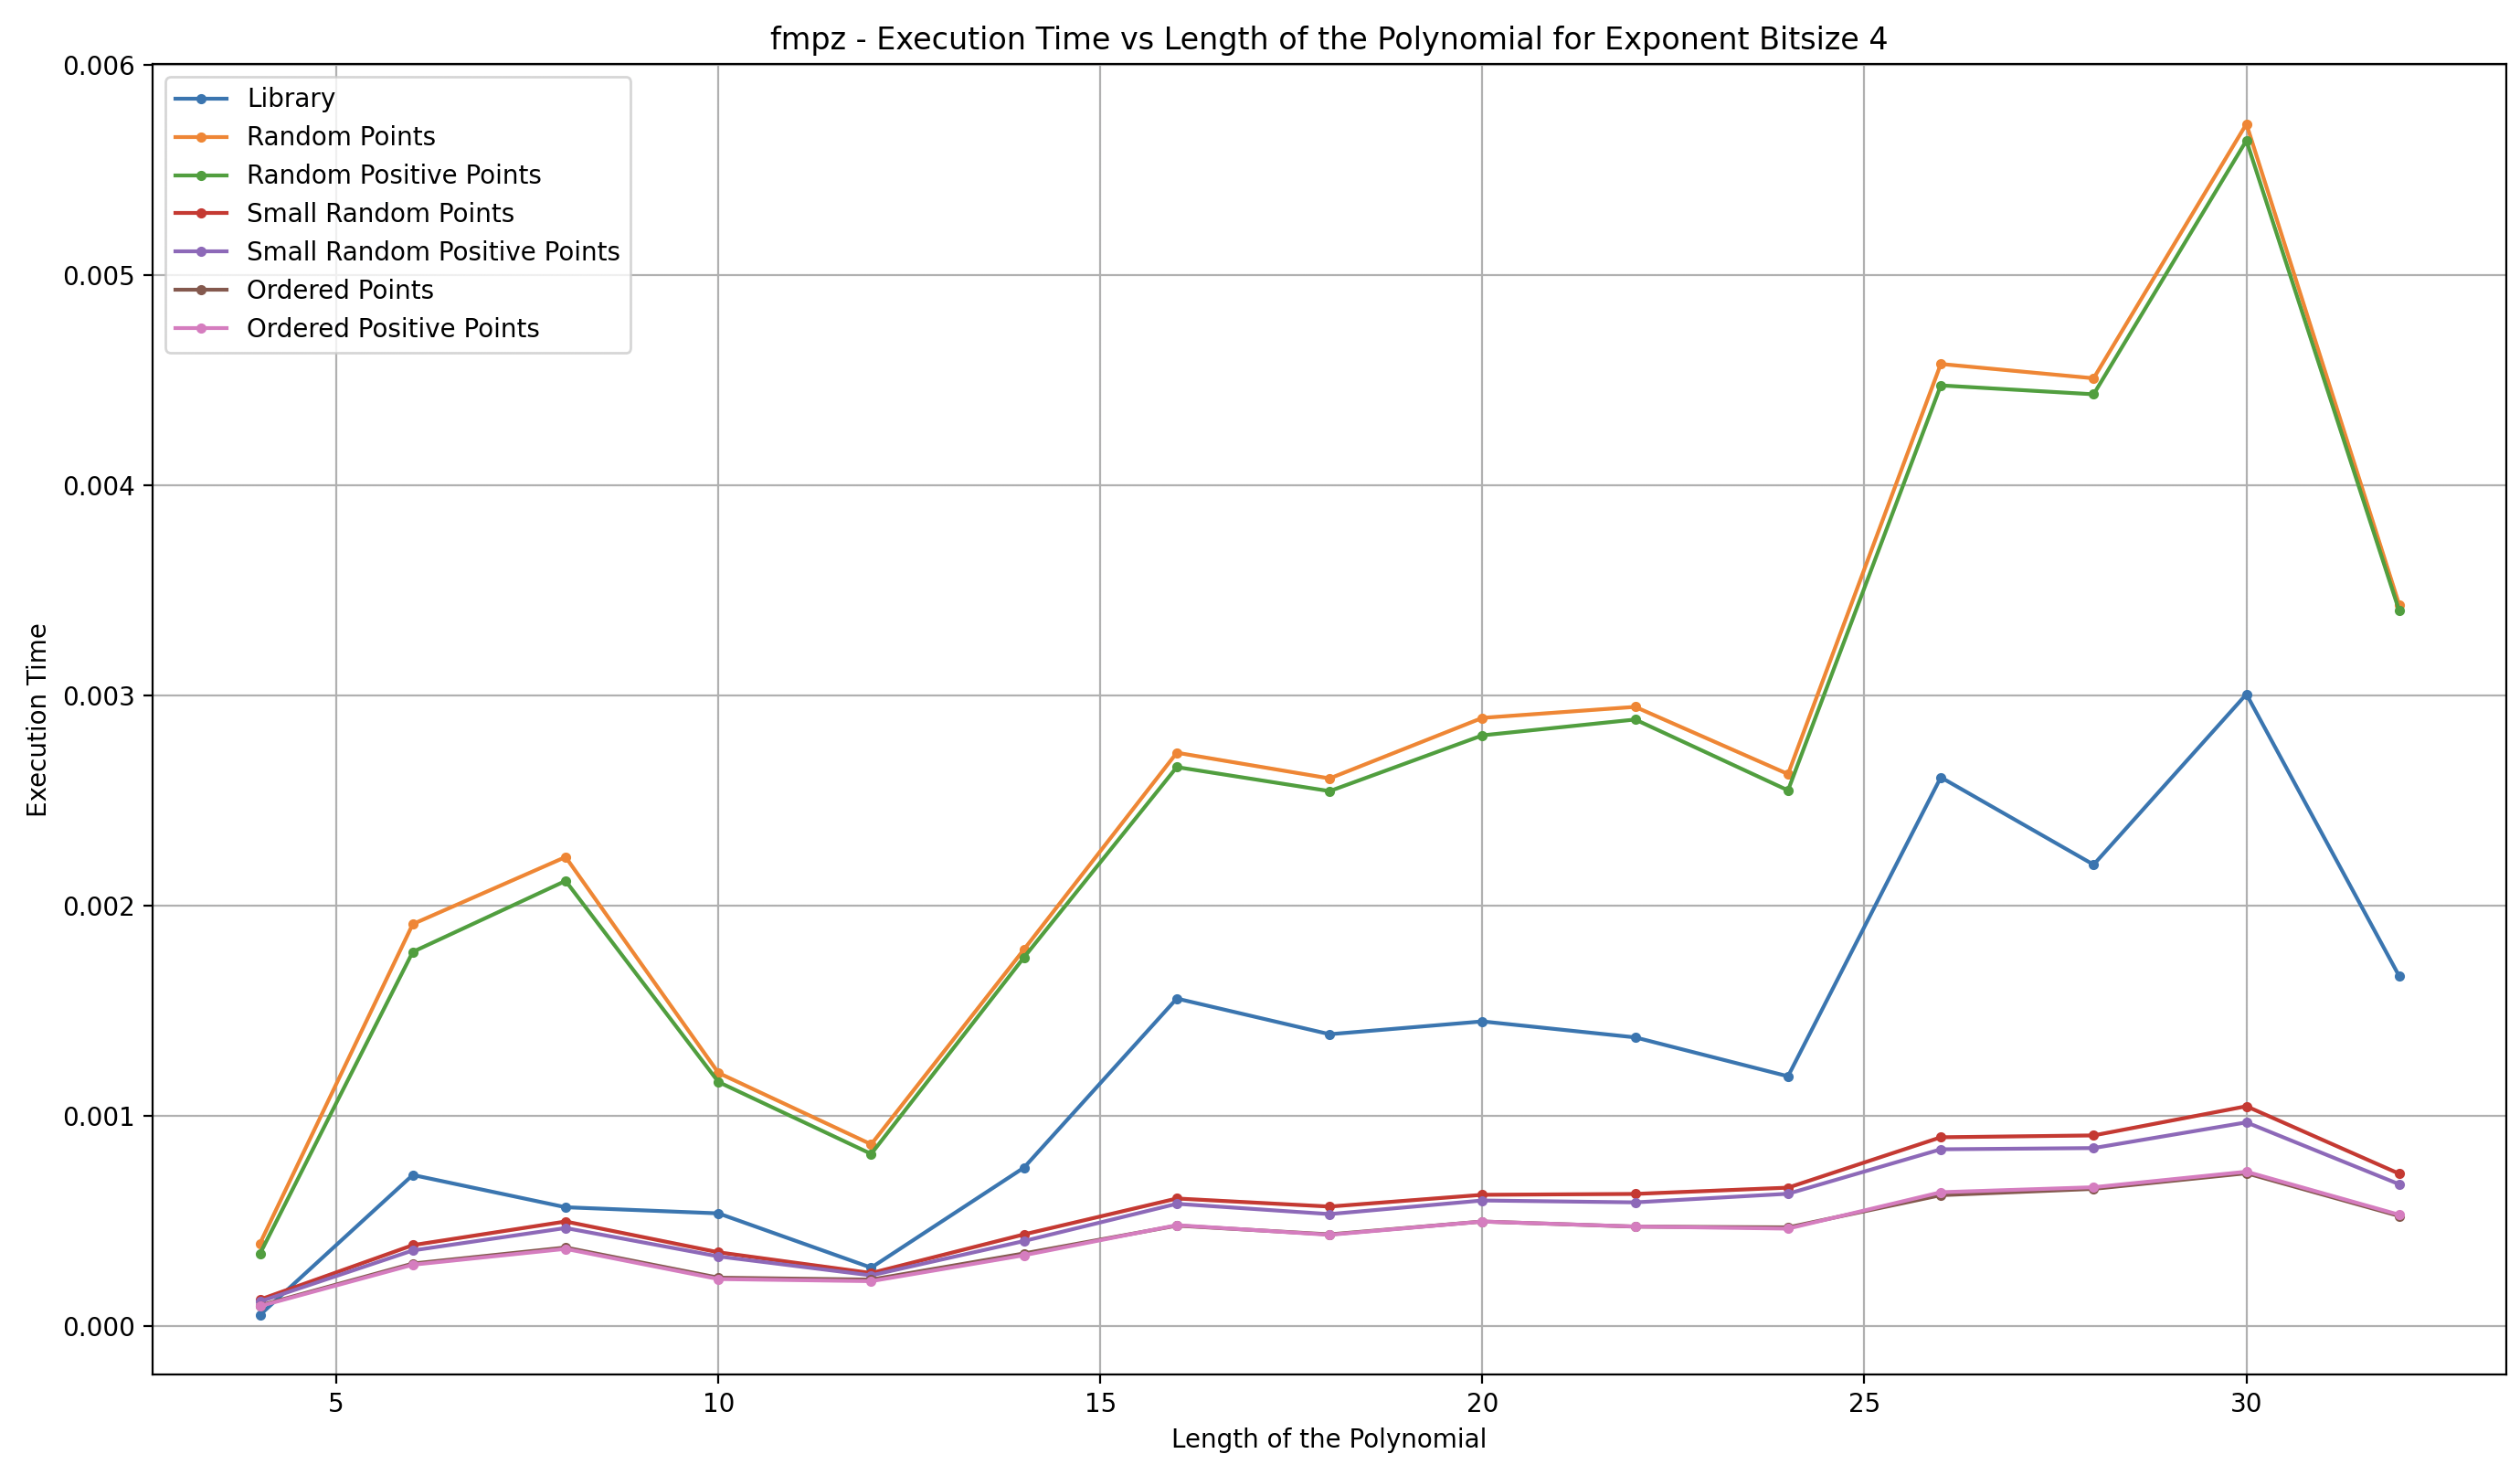
\includegraphics[width=\linewidth]{./images/fmpz_bitsize_4.png}
    \caption{FMPZ bivariate polynomial resultant execution time (in seconds) for exponent bitsize 4 with varying lengths.}
    \label{fig:benc.fmpz.4}
  \end{subfigure}%
  \hspace{0.05\textwidth}%
  \begin{subfigure}{0.45\textwidth}
    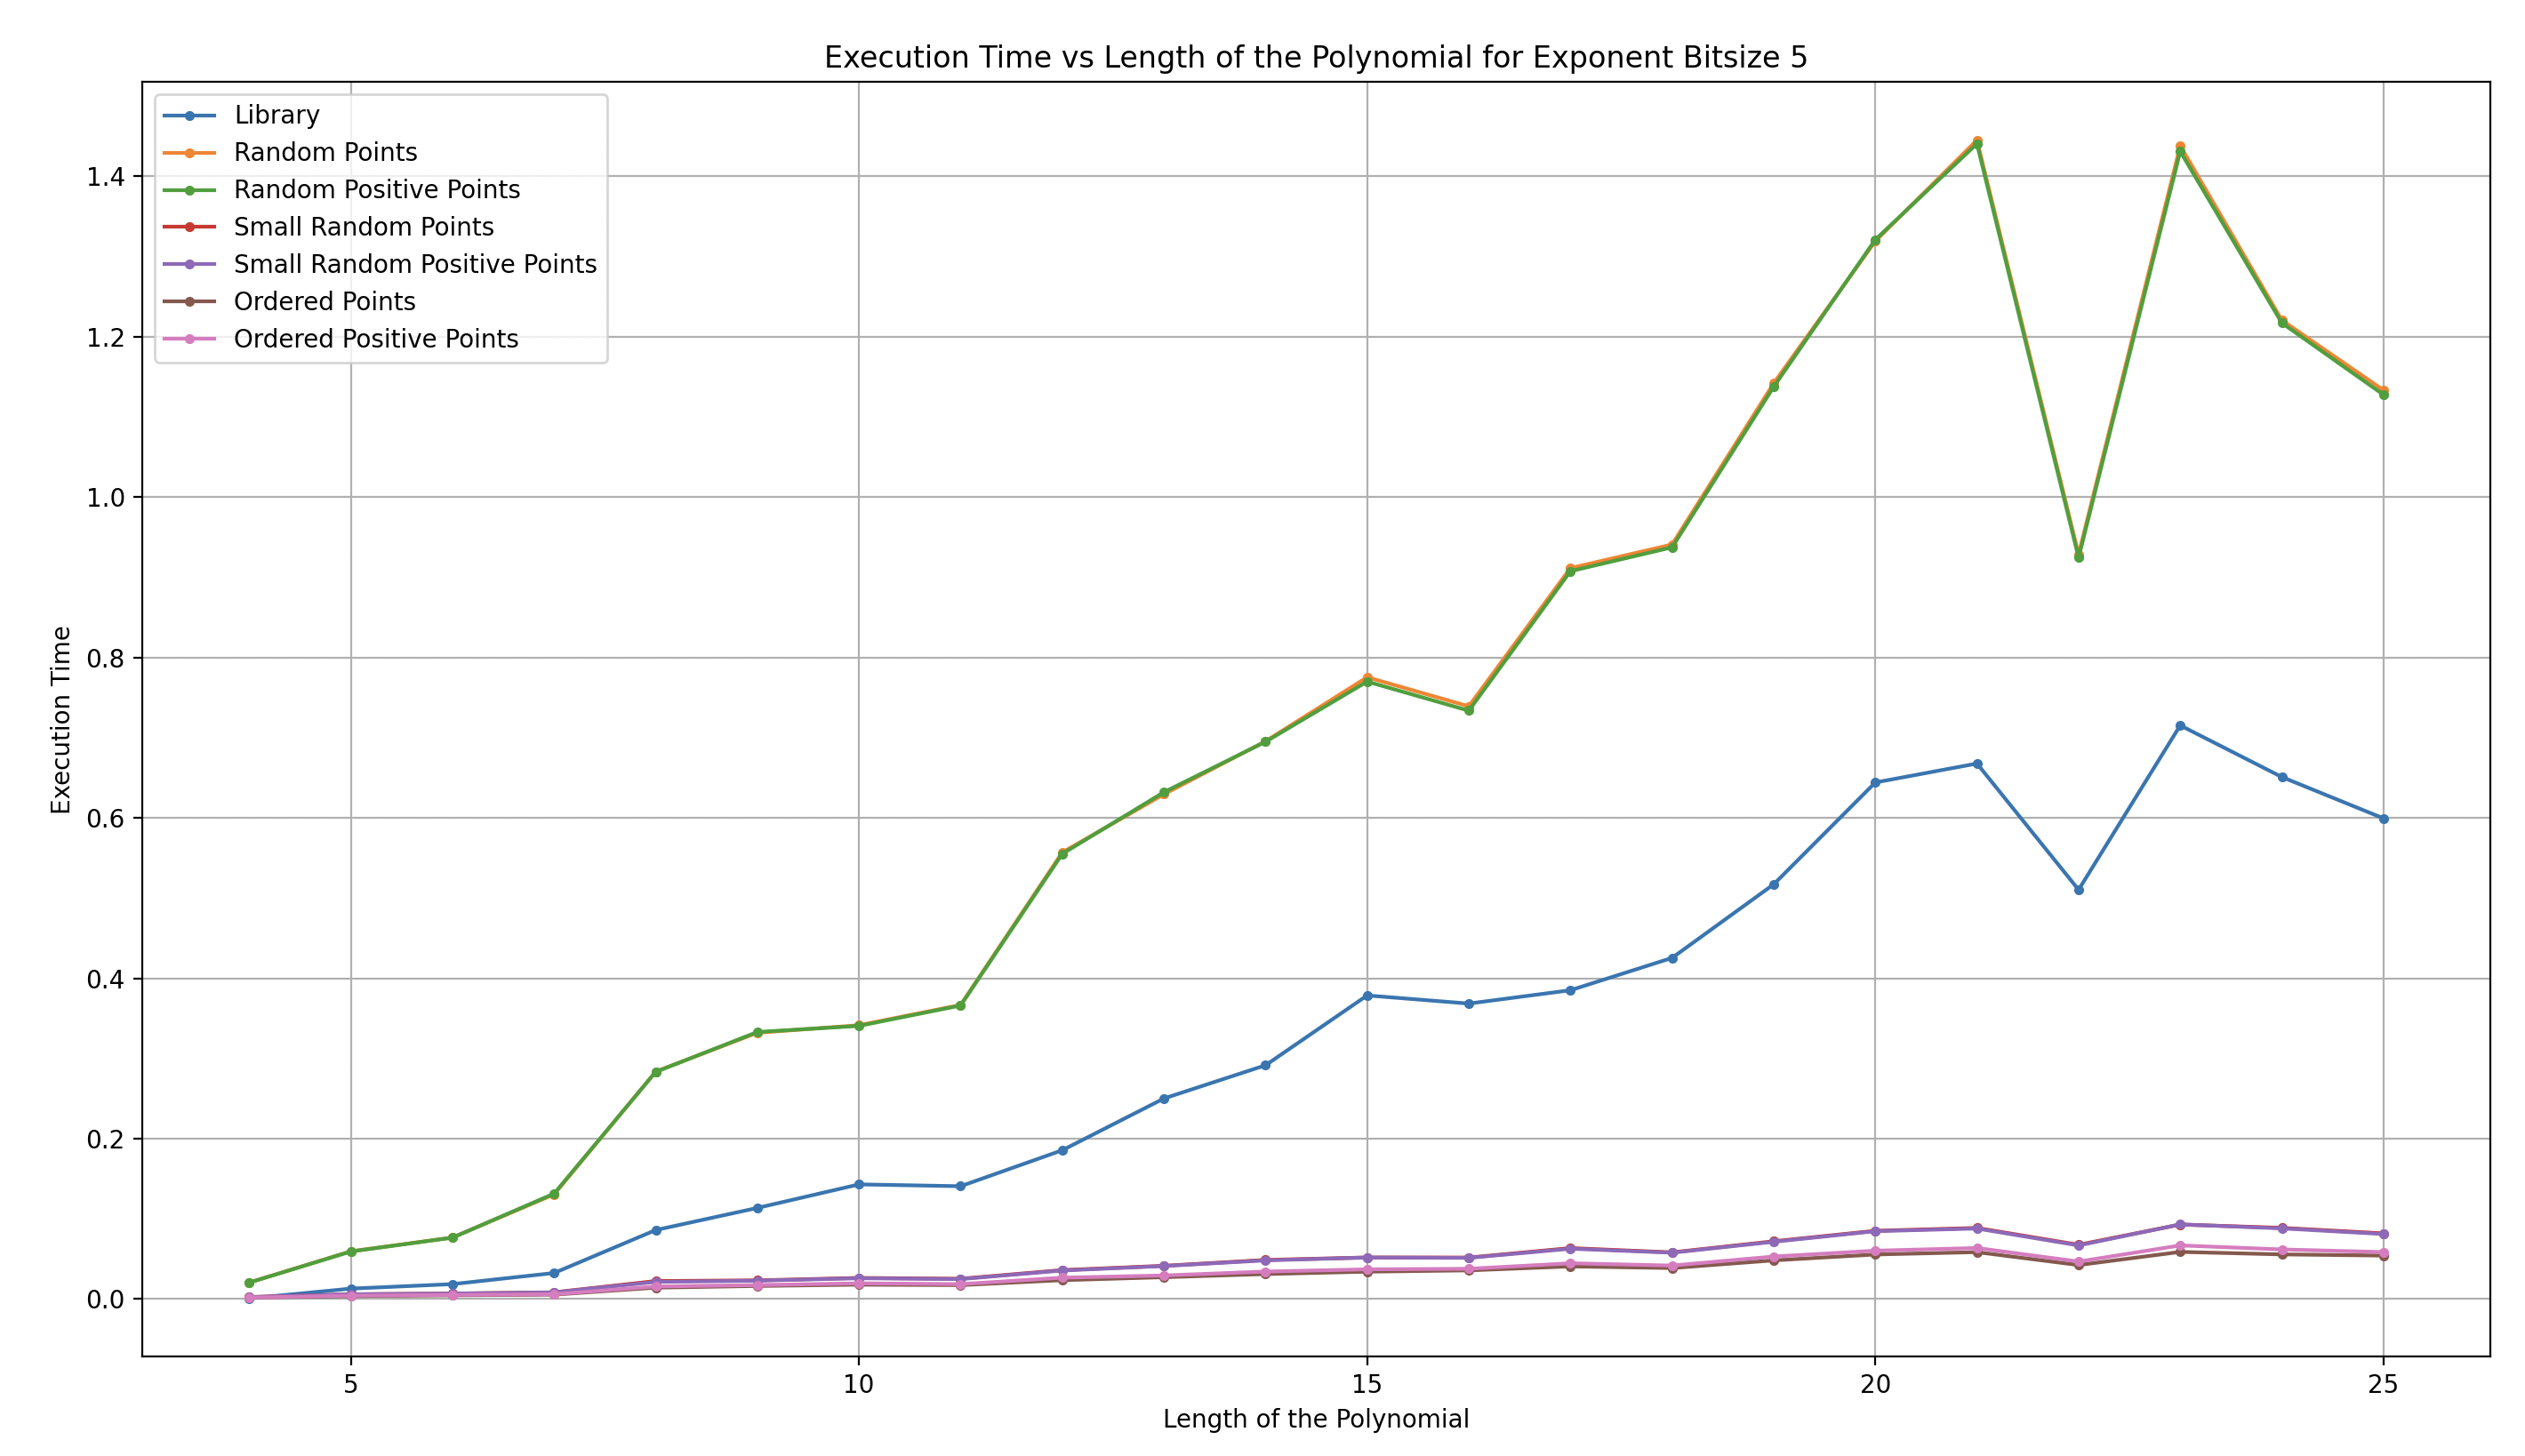
\includegraphics[width=\linewidth]{./images/fmpz_bitsize_5.png}
    \caption{FMPZ bivariate polynomial resultant execution time (in seconds) for exponent bitsize 5 with varying lengths.}
    \label{fig:benc.fmpz.5}
  \end{subfigure}
\end{figure}

In Figure \ref{fig:benc.fmpz.4} and \ref{fig:benc.fmpz.5}, we extend our analysis to bigger polynomials with the exponent bitsize 4 and 5, respectively. We see that the relation between the random selection method and other categories is still the same, while the difference between the FLINT library implementation and our methods starts to become visible. As the length of polynomials increase, FLINT performs much slower than our algorithm. Notice also that there is not too much difference between randomly selecting interpolation points with small bitsize and having them ordered in the bitsize, which supports our intiution that the running time of polynomial interpolation depends on the bitsize of selected points.

Moreover, we can observe that all curves follow a similar shape with considerable fluctuations. Even though the overall trend is that increasing the polynomial's length increases the running time, we see that for some lengths there is a sharp decrease in the measure time. This result can be explained by the properties of the random bivariate polynomial generation function of FLINT. For some testcases, the generated polynomials have a resultant that is much harder to compute. This fluctuation can be minimized by increasing number of trials per length, but since our main motivation is comparing different methods, but not giving an accurate estimate of their dependence of the length of the polynomial, we keep this methodology.

\begin{figure}[H]
  \centering
  \begin{subfigure}{0.5\textwidth}
    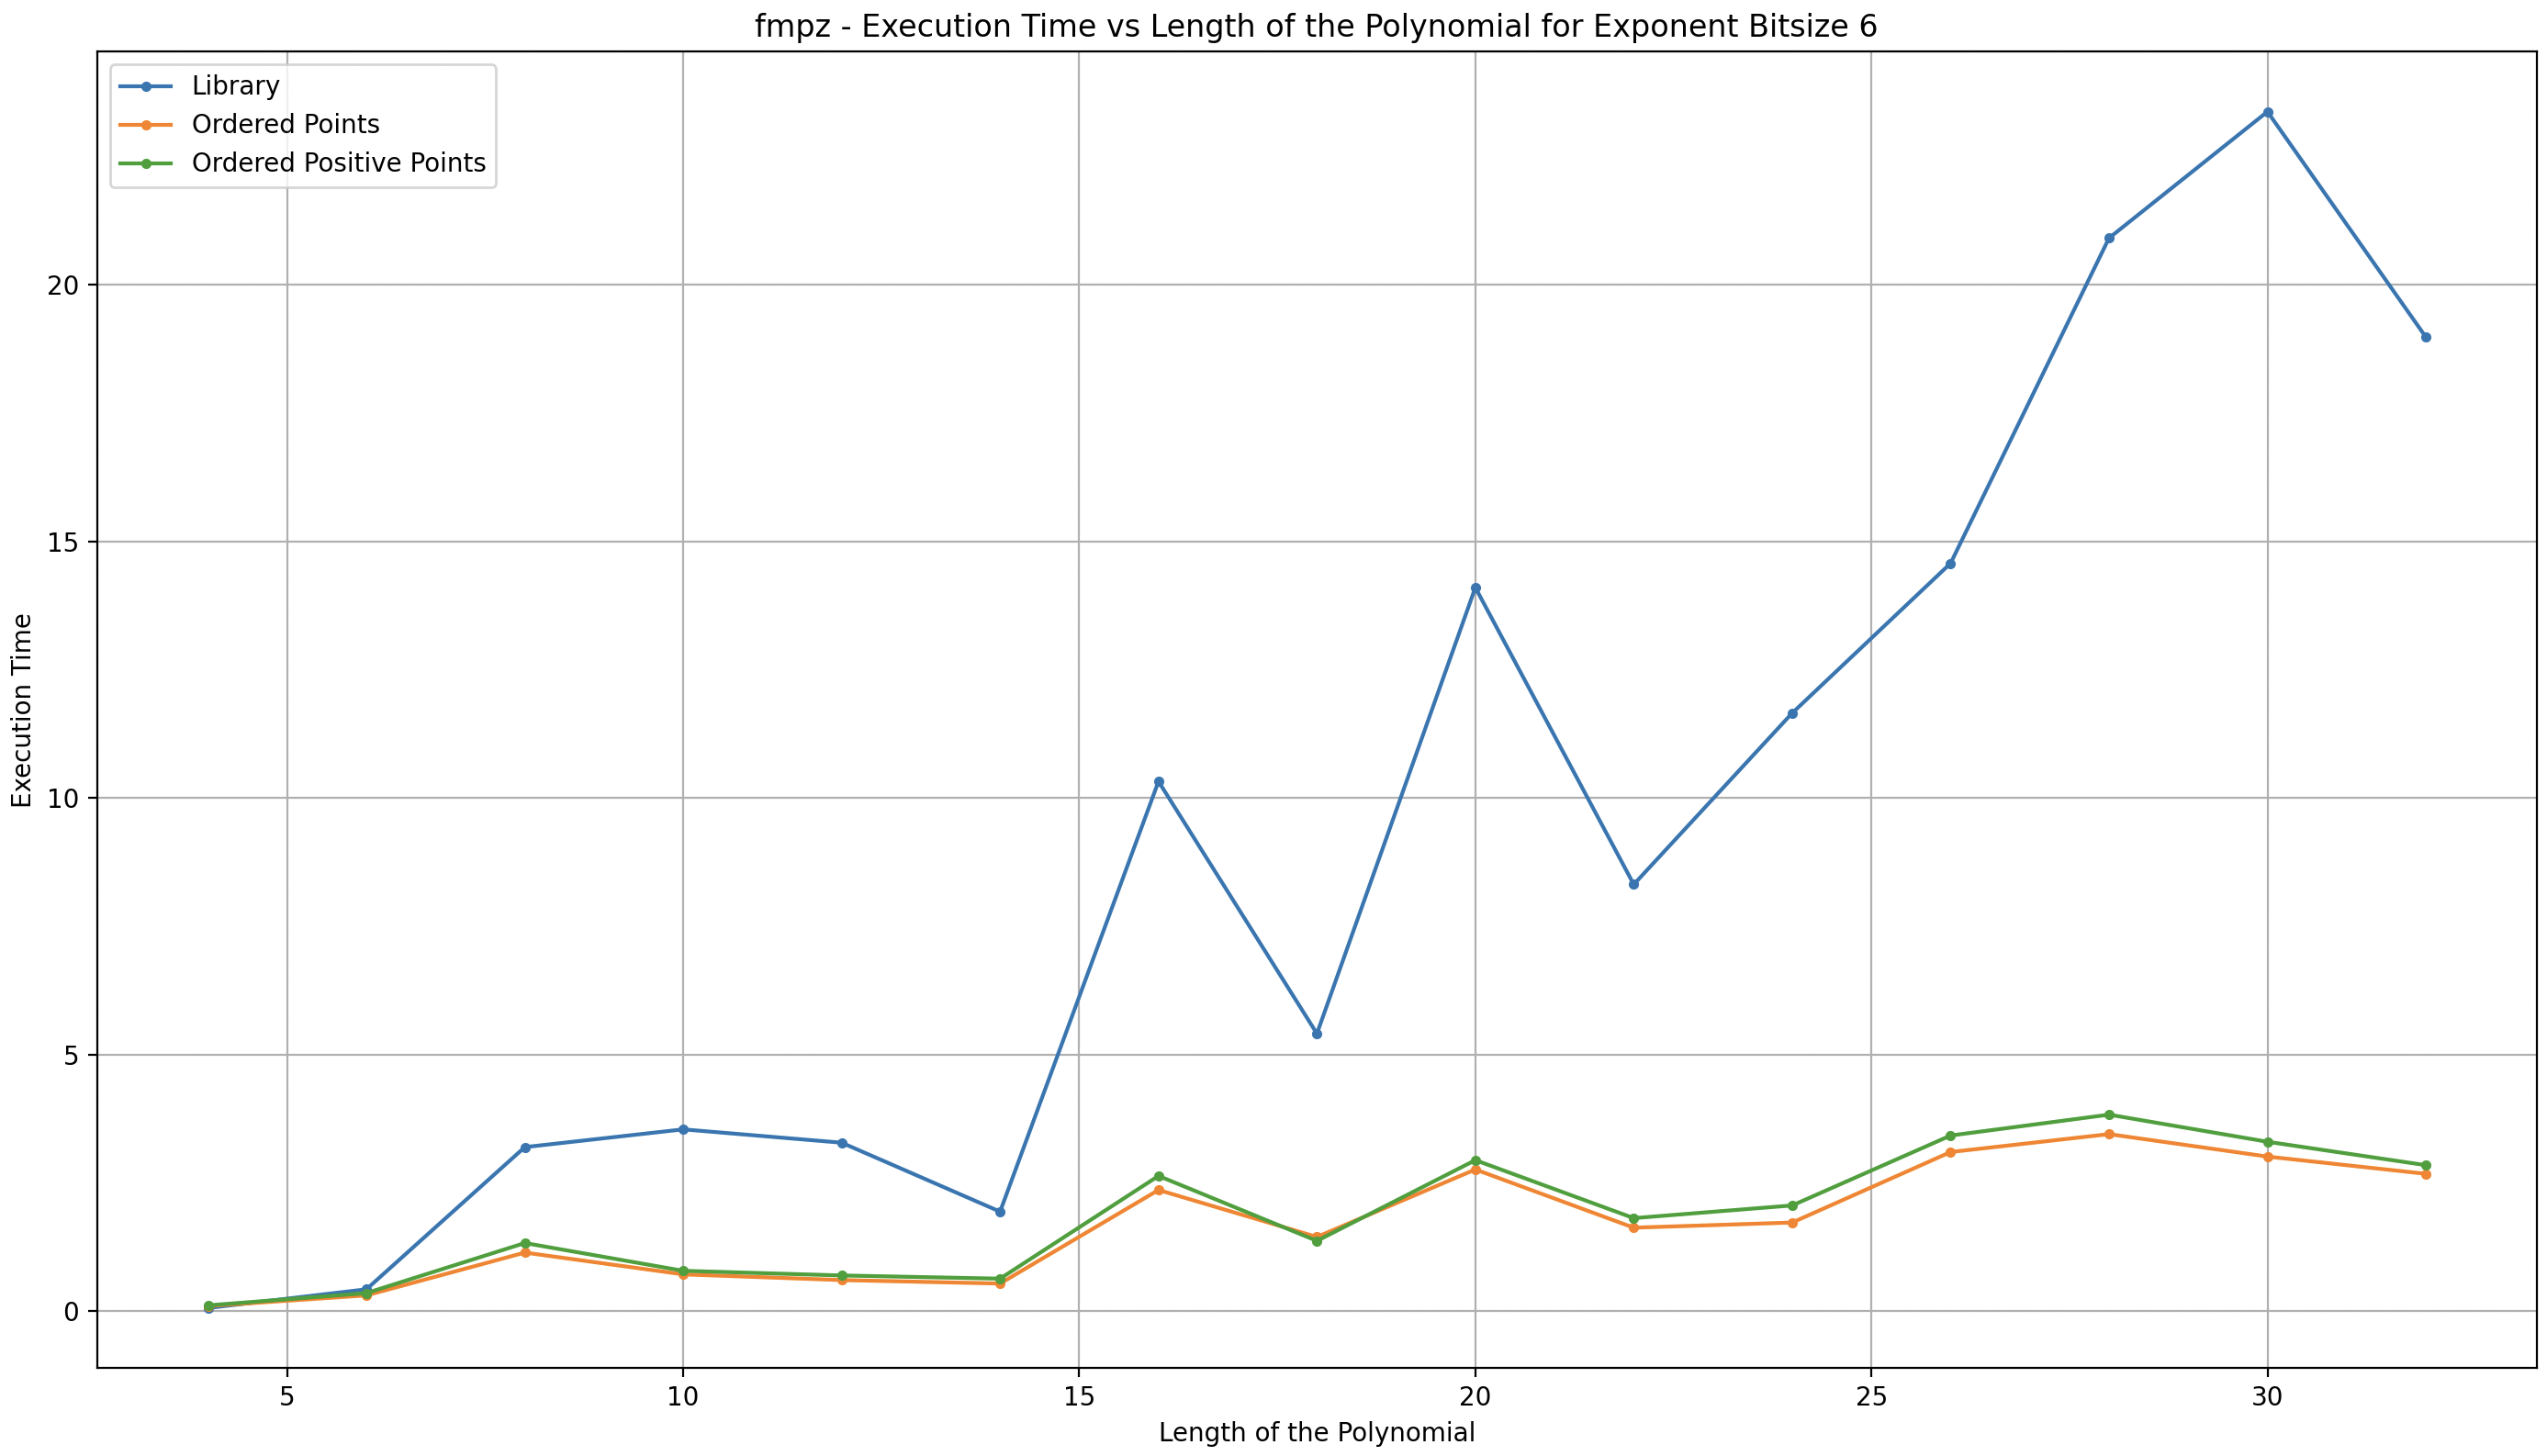
\includegraphics[width=\linewidth]{./images/fmpz_bitsize_6.png}
  \end{subfigure}
  \caption{FMPZ bivariate polynomial resultant execution time (in seconds) for exponent bitsize 6 with varying lengths.}
  \label{fig:benc.fmpz.6}
\end{figure}

Finally, we measure with polynomials of the exponent bitsize 6, where we only include the library and ordered implementations to minimize the total running time. We observe that the difference between both methods becomes even more important, where we achieve an approximate of $7 \times$ performance increase compared to FLINT. For bigger bitsizes, total running times exceeds 30 seconds for a single measurement, thus we do not present the results here.

\subsection{Benchmarks for rational polynomials}

In this section, we extend our analysis to polynomials over $\mathbb{Q}$ instead of $\mathbb{Z}$, but note that presented results do not really differ from what we have observed for $\mathbb{Z}$. Interpolation using random points with big bitsize is significantly slower than rest of the methods, and the FLINT implementation starts becoming much slower than our implementations as the exponent bitsize and the length of the polynomials increase. Using ordered points in bitsize for interpolation is slightly more performant than using random points with small bitsize, but both methods are still significantly faster than FLINT. The maximum achieved performance improvement is again around $7 \times$ compared to FLINT.

\begin{figure}[H]
  \centering
  \begin{subfigure}{0.45\textwidth}
    
\includegraphics[width=\linewidth]{./images/fmpq_bitsize_3.png}
    \caption{FMPQ bivariate polynomial resultant execution time (in seconds) for exponent bitsize 3 with varying lengths.}
    \label{fig:benc.fmpq.3}
  \end{subfigure}%
  \hspace{0.05\textwidth}%
  \begin{subfigure}{0.45\textwidth}
    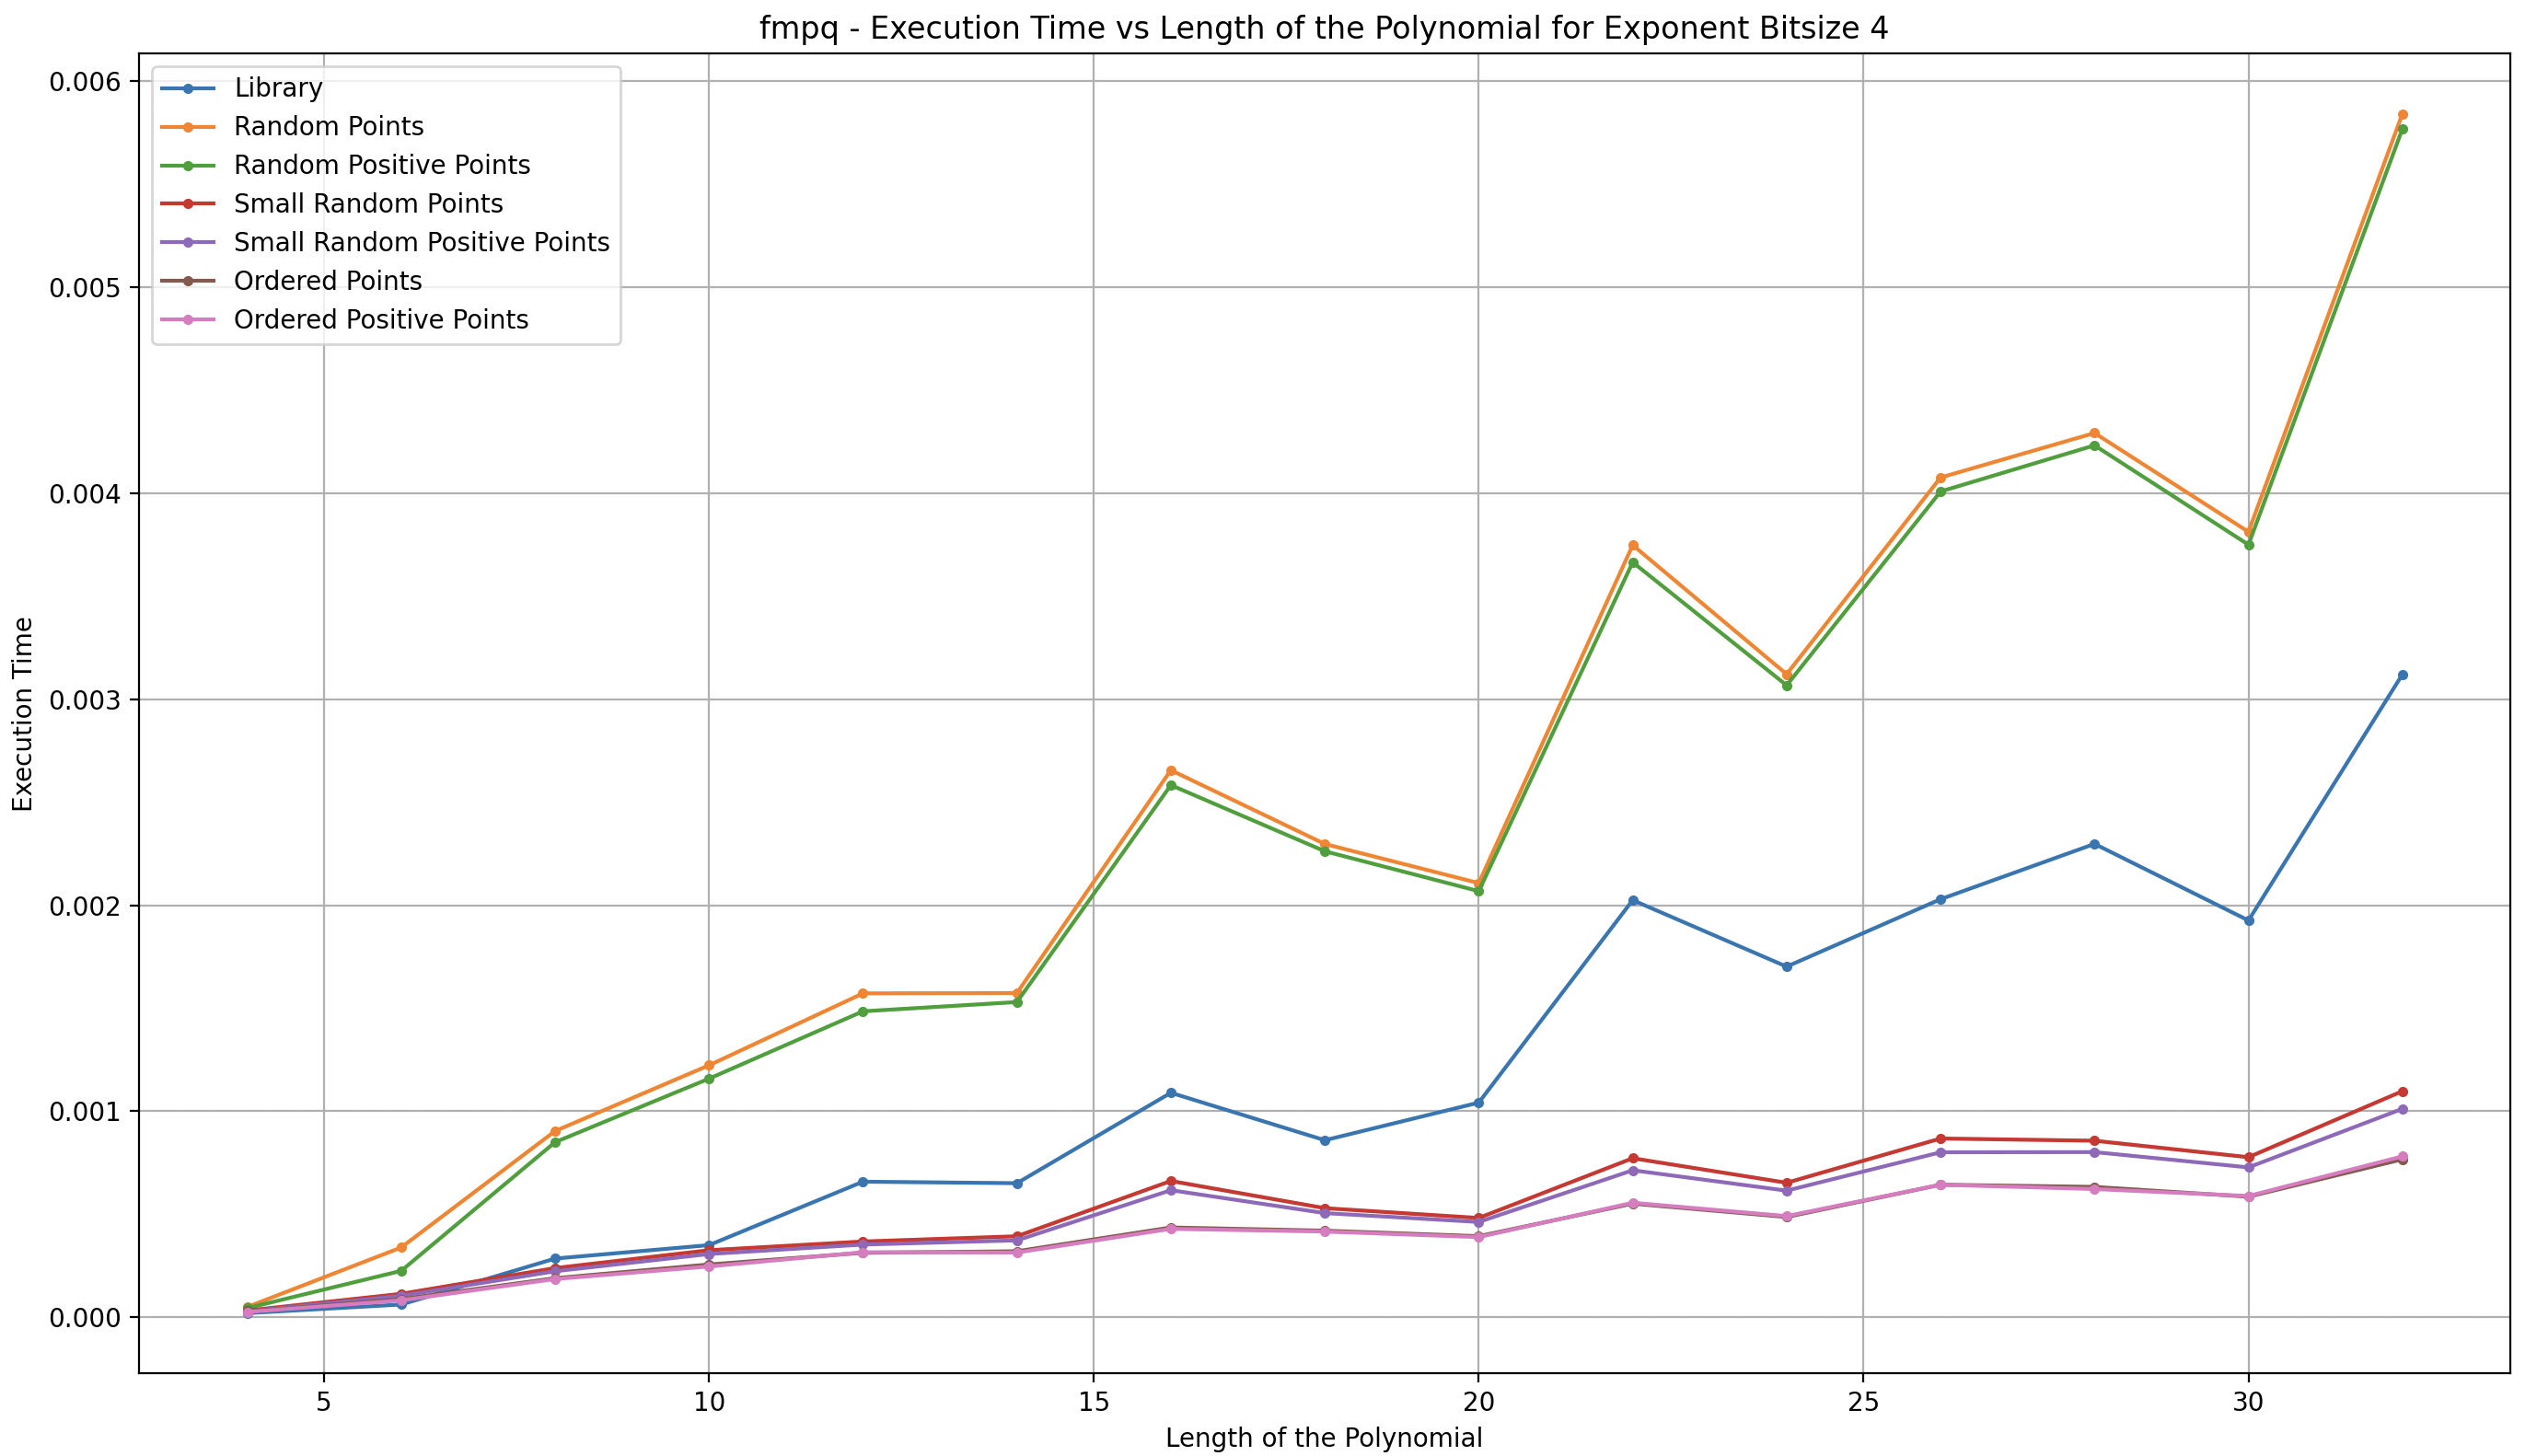
\includegraphics[width=\linewidth]{./images/fmpq_bitsize_4.png}
    \caption{FMPQ bivariate polynomial resultant execution time (in seconds) for exponent bitsize 4 with varying lengths.}
    \label{fig:benc.fmpq.4}
  \end{subfigure}
\end{figure}

\begin{figure}[H]
  \centering
  \begin{subfigure}{0.45\textwidth}
    
\includegraphics[width=\linewidth]{./images/fmpq_bitsize_5.png}
    \caption{FMPQ bivariate polynomial resultant execution time (in seconds) for exponent bitsize 5 with varying lengths.}
    \label{fig:benc.fmpq.5}
  \end{subfigure}%
  \hspace{0.05\textwidth}%
  \begin{subfigure}{0.45\textwidth}
    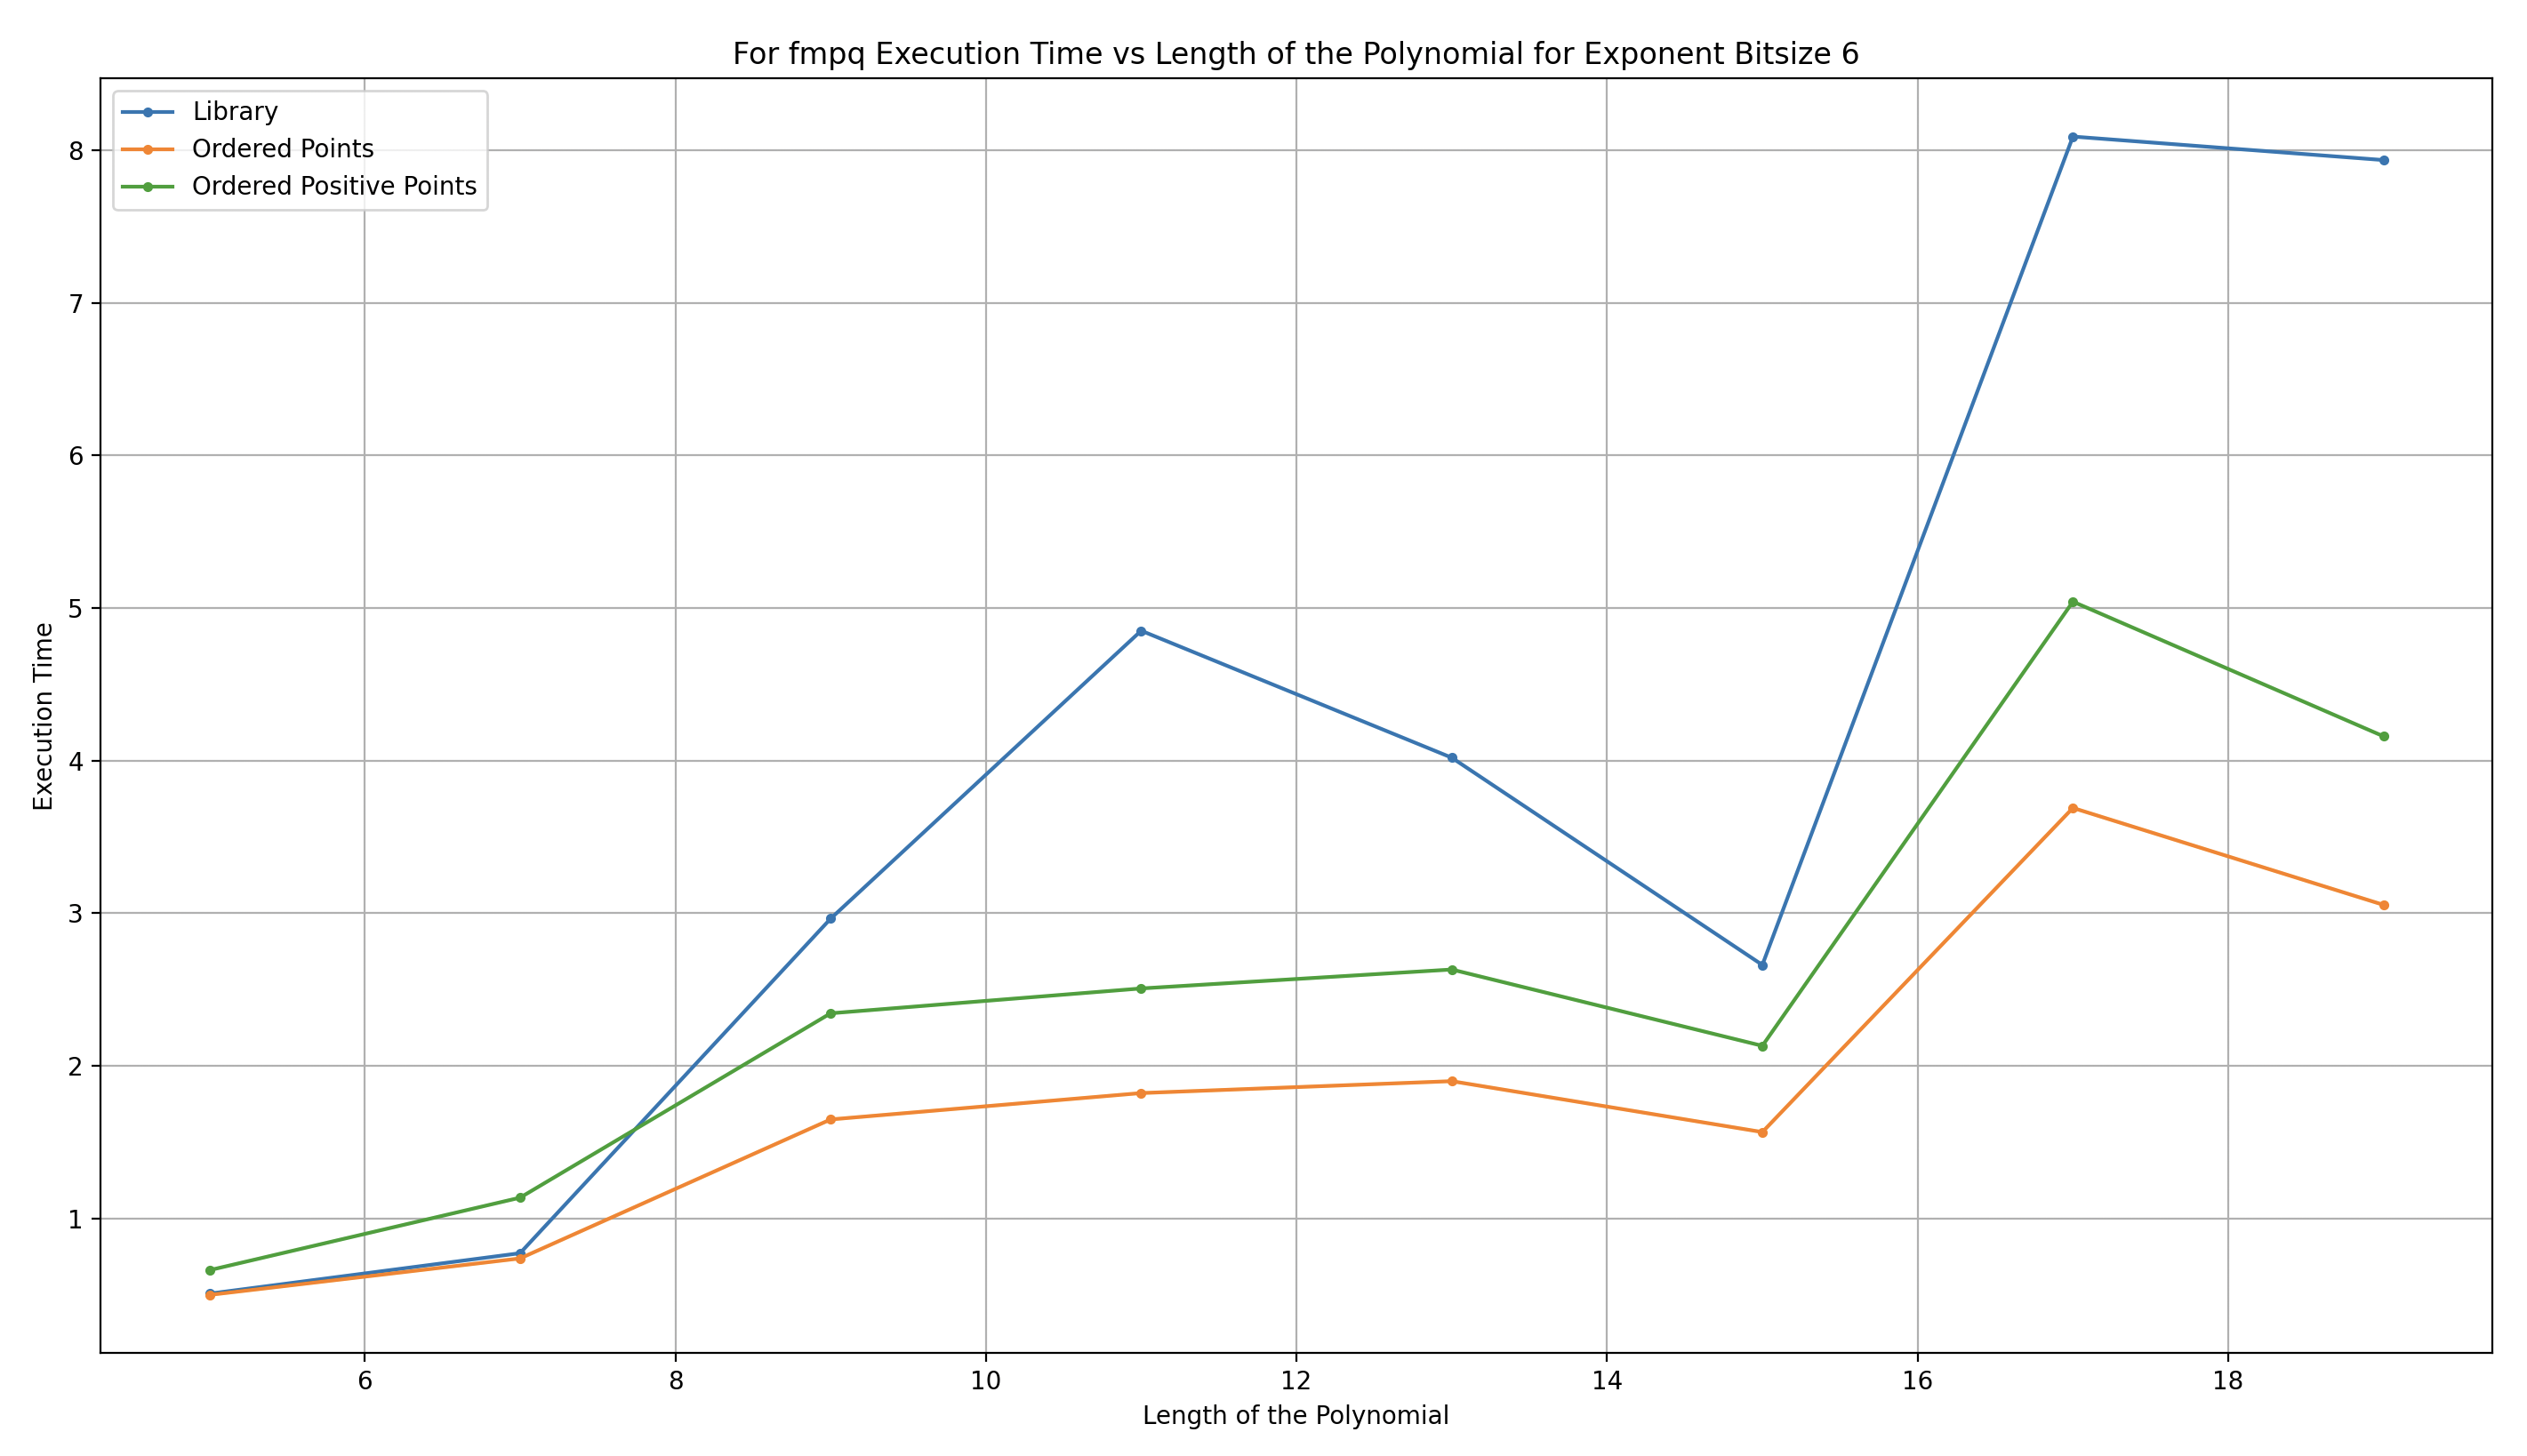
\includegraphics[width=\linewidth]{./images/fmpq_bitsize_6.png}
    \caption{FMPQ bivariate polynomial resultant execution time (in seconds) for exponent bitsize 6 with varying lengths.}
    \label{fig:benc.fmpq.6}
  \end{subfigure}
\end{figure}
